\documentclass[chapter,a4paper,10pt]{oblivoir}

\usepackage[margin=24mm]{geometry}
\usepackage{graphicx}
\usepackage{relsize}
\usepackage{amsmath}
\usepackage{bm}
\usepackage{url}

\begin{document}

\title{회귀분석(Regression Analysis)}
\author{이정우\\phyjics@gmail.com}
\maketitle
\tableofcontents

\chapter{최소 제곱법(Least Squares Fitting)}

\section{선형 회귀 - 직선}

N개의 데이터 점$(x_i, y_i)$이 직선
\begin{equation}
f(x) = ax + b,
\end{equation}
의 분포를 따른다고 할 때 최소 제곱법은 데이터와 직선 사이의 $y$값 차이를 제곱하여 합한 값을 최소화 하는 방법이다.
최소화 하고자 하는 값 $S$는 다음과 같다.
\begin{equation}
S = \sum_{i=1}^N (y_i - ax_i - b)^2.
\end{equation}
이를 변수 $a$와 $b$에 대해서 각각 최소화 하면;
\begin{equation}
\frac{\partial S}{\partial a} = 0,\,\,\,\, \frac{\partial S}{\partial b} = 0,
\end{equation}
아래와 같이 $a$와 $b$를 구할 수 있다.
\begin{eqnarray}
a
%&=&\frac{N\sum x_i y_i - \sum x_i \sum y_i}{N\sum x_i^2 - (\sum x_i)^2}.
&=& \frac{\langle x_i y_i \rangle - \langle x_i \rangle \langle y_i\rangle}{\langle x_i^2 \rangle - \langle x_i \rangle^2}.
\\\nonumber\\
b
%&=& \frac{\sum x_i^2 \sum y_i - \sum x_i \sum x_i y_i}{N\sum x_i^2 - (\sum x_i)^2}.
&=& \frac{\langle x_i^2 \rangle \langle y_i \rangle - \langle x_i \rangle \langle x_i y_i\rangle}{\langle x_i^2 \rangle- \langle x_i\rangle^2}.
\end{eqnarray}

%\begin{eqnarray}
%\sigma_y^2 &=& \sum_{i=1}^N P_i (y_i - ax_i - b)^2\\
%           &=& \frac{1}{N}\sum_{i=1}^N (y_i - ax_i - b)^2
%\end{eqnarray}

\section{함수를 알고 있는 경우}

N개의 데이터 점$(x_i, y_i)$이
\begin{equation}
f(x) = av(x-b),
\end{equation}
의 분포를 따른다고 할 때 최소화 하고자 하는 $S$는
\begin{equation}
S = \sum_{i=1}^N \left(y_i - av(x_i - b)\right)^2,
\end{equation}
이 된다. 이를 $a$와 $b$에 대해서 최소화 하면
(${\partial S}/{\partial a} = 0,\,\,{\partial S}/{\partial b} = 0$)
다음과 같다.
\begin{eqnarray}
\frac{\partial S}{\partial a} = 0 &\longrightarrow& a = \frac{\sum y_i v(x_i - b)}{\sum f^2(x_i - b)}.%,\\\nonumber\\
\end{eqnarray}
함수의 형태를 알지 못할 떄 변수 $b$는 함수 $v$에 종속되어 있어 구할 수 없다. 하지만 특정 $b$에서 최소 제곱법에 맞는 $a$를 구할 수 있다.
함수의 형태를 알고 있을 때는 경우에 따라 다음 식을 이용하여 $b$를 구할 수 있다.
\begin{eqnarray}
\frac{\partial s}{\partial b} = 0 &\longrightarrow& a = \frac{\sum y_i v'(x_i - b)}{\sum v(x_i - b)v'(x_i - b)}\\\nonumber\\
&&v'(x) \equiv \frac{\partial v(x)}{\partial x}
\end{eqnarray}

\chapter{원 피팅}
\section{리만 피팅}
\subsection{극사영}
극사영은(stereographic projection)은 구면의 점을 평면으로,
또는 반대로 옮기는 합수이며 입체사영(conformal mapping)으로도 불린다.
$(x,z)$ 평면위의 점 $\textrm P_i(x_i,0,z_i)$와, 원점 O$(0,0,0)$ 위에 놓인
리만 구(Riemann sphere) S를 생각해보자.
이 구는 $R$의 반지름을 가지며 중심점 C는 $(0, R, 0)$로 주어진다.
\begin{equation}
\textrm{S} \,\,:\,\, x^2 + (y-R)^2 + z^2 = R^2
\end{equation}
점 $\textrm P_i$에서 리만 구의 꼭지점 T$(0,2R,0)$를 잇는 선이
구와 만나는 점을 $\textrm P_i'$$(x_i',y_i',z_i')$라고 하자.
반지름 $r_i$를 $r_i \equiv {\sqrt{x_i^2 + z_i^2}}/{2R}$ 와 같이 정의 하였을 때
점 $\textrm P_i'$는 점 $\textrm P_i$로 부터 다음과 같이 주어진다.
\begin{eqnarray} \label{XDataToXMap}
x_i' &=& \frac{x_i}{1 + r_i^2} \\
y_i' &=& \frac{2Rr_i^2}{1 + r_i^2} \nonumber\\
z_i' &=& \frac{z_i}{1 + r_i^2} \nonumber
\end{eqnarray}
반대로 점 $\textrm P_i$는 점 $\textrm P_i'$로 부터 다음과 같이 주어진다.
\begin{eqnarray}
x_i &=& \frac{x_i'}{1 - y_i'/2R} \\
z_i &=& \frac{z_i'}{1 - y_i'/2R} \nonumber
\end{eqnarray}
\subsection{리만 구 위의 원}
리만 구 위에 사영된 데이터 점 $\textrm P_i'$을 평면으로 피팅을 하였을 때(\ref{section_fitplane}절 참조)
구해진 평면 K의 수직 벡터를 $\mathbf{n}(a,b,c)$, 평면에 속한 한점($\textrm P_i'$의 평균)을
M$(\langle x\rangle',\langle y\rangle',\langle z\rangle')$이라 하자.
\begin{equation}
\textrm{K} \,\,:\,\, a(x-\langle x\rangle') + b(y-\langle y\rangle') + c(z-\langle z\rangle') = 0
\end{equation}
평면이 구를 자르면서 생기는 원의 중심점 A는 리만구의 중심점 C를 지나고
$\mathbf{n}$의 방향을 가진 직선 L이 평면 K와 만나는 점이 된다.
\begin{equation}
\textrm{L} \,\,:\,\,
\left\{
\begin{array}{ll}
x = at \\
y = bt + R\\
z = ct
\end{array}
\right.
\end{equation}
연립하여 풀면 중심점에서의 $t$인 $t_A$는 다음과 같고
\begin{equation}
t_A = \frac{a\langle x\rangle'+ b(\langle y\rangle'-R) + c\langle z\rangle'} {a^2 + b^2 + c^2},
\end{equation}
원의 중심점 $\textrm{C}_\textrm{A}$는 $(at_A, bt_A + R, ct_A)$이 되며
리만 구의 중심에어 원의 중심까지의 거리가 $l = |\overline{\textrm{CC}}_\textrm{A}|$ 일때
원의 반지름 $r_A$는 $\sqrt{R^2 - l^2}$이 된다.
\subsection{역 극사영}
원 A를 $xz$평면 위에 뉘고($\textrm{A}_\perp,\mathbf{x}_\perp$)
\begin{equation}
\textrm{A}_\perp \,\,:\,\, x_\perp^2 + z_\perp^2 = r_A^2
\end{equation}
벡터 $\hat{\mathbf{y}}$가 피팅한 평면의 수직벡터$\mathbf{n}$과 같도록 회전시킨 후
$y$ 방향으로 $(\textrm{C}_\textrm{A})_y$ 만큼 올린 원이 된다.
회전 행렬 $\mathbf{R}$을 $x$축, $y$축으로 분리해서 보자.
\begin{equation}
\mathbf{R} = \mathbf{R_y(\phi)}\mathbf{R_x(\theta)},
\end{equation}
\begin{equation}
\mathbf{R_y(\phi)} = \left( \begin{array}{ccc}
  \cos \phi & 0 & \sin \phi \\
  0 & 1 & 0 \\
  -\sin \phi & 0 & \cos \phi
\end{array} \right) ,\,\,\,
\mathbf{R_x(\theta)} = \left( \begin{array}{ccc}
  1 & 0 & 0 \\
  0 & \cos \theta & -\sin \theta \\
  0 & \sin \theta & \cos \theta
\end{array} \right)
\end{equation}
이 회전은 $\hat{\mathbf{y}}$가 $\mathbf{n}$가 되는 회전과 같다.
\begin{equation}
\mathbf x' = \mathbf R\mathbf x_\perp
\,\,\,\longrightarrow\,\,\,\,\,
\mathbf{R} \hat{\mathbf{y}} = \mathbf{n},
\end{equation}
따라서 다음과 같이 행렬의 각 성분들을 구할 수 있다.
\begin{equation}
\left. \begin{array}{ll}
\cos \theta = b \\
\sin \theta = d \\
\cos \phi = c/d \\
\sin \phi = a/d \\
\end{array}\right.
\,\,\,,\,\,\,\,\,\,\,d \equiv \sqrt{1-b^2}
\end{equation}
이 되고 $\mathbf{R}$, $\mathbf{R}^{-1}$과 변환 식은 다음과 같이 쓸 수 있다.
\begin{equation}
\mathbf{R} = \left( \begin{array}{ccc}
  c/d & a & ab/d \\
  0 & b & -d \\
  -a/d & c & bc/d
\end{array} \right)
,\,\,\,\mathbf{R}^{-1} = \left( \begin{array}{ccc}
  c/d & 0 & -a/d \\
  a & b & c \\
  ab/d & -d & bc/d
\end{array} \right)
\end{equation}
\begin{eqnarray}
&&\mathbf{x}_\perp\rightarrow\mathbf{x}'\,\,\,
\left\{ \begin{array}{ll}
x' = ({c}/{d})x_\perp + ay_\perp + ({ab}/{d})z_\perp\\
y' = by_\perp - dz_\perp\\
z' = -({a}/{d})x_\perp + cy_\perp + ({bc}/{d})z_\perp
\end{array} \right.\\
\nonumber\\
&&\mathbf{x}'\rightarrow\mathbf{x}_\perp\,\,\,
\left\{ \begin{array}{ll}
x_\perp = ({c}/{d})x' - ({a}/{d})z'\\
y_\perp = ax' + by' + cz'\\
z_\perp = ({ab}/{d})x' - dy' + ({bc}/{d})z'
\end{array} \right.
\end{eqnarray}
원 $\textrm{A}_\perp$를 변환식을 통하여 치환하고
$y$ 방향으로 $(\textrm{C}_\textrm{A})_y$ 만큼 올리면 다음과 같다.
\begin{equation}
\left(cx' - az'\right)^2 + \left(abx' - d^2(y'-(\textrm{C}_\textrm{A})_y) + bcz'\right)^2 = r_A^2d^2
\end{equation}
다음으로 식 (\ref{XDataToXMap}) 을 이용하여 리만구의 원을 $xz$ 평면으로 옮겨 보자.
\begin{equation}
\left(cx - az\right)^2 + \left(abx - d^2\left(2Rr^2-(1+r^2)(\textrm{C}_\textrm{A})_y\right) + bcz\right)^2 = \left(r_Ad(1+r^2)\right)^2
\end{equation}
그런데 이렇게 계산하다보면 끝이 나지 않는다! 이럴수가! 살려줘!

\subsection{역 극사영 초콜릿 먹고싶다}
작전은 이렇다. 원 A에서 $y$ 값이 가장 작은 점과 가장 큰 점을 구해서 역 극사영 시킨다.
이 두점은 역 극사영 된 후에도 서로 원의 정 반대편에 위치하므로
$xz$ 평면에서의 최종 원을 쉽게 구할 수 있다.
중심점은 두 점의 중간지점이고 반지름은 두 점 사이 거리의 반이다!
오! 된다! 코딩해봤더니 됩니다!
\begin{equation}
\mathbf{R}' = \mathbf{R_y(\phi)}\mathbf{R_x(\alpha)},
\end{equation}
\begin{equation}
\mathbf{R_y(\phi)} = \left( \begin{array}{ccc}
  \cos \phi & 0 & \sin \phi \\
  0 & 1 & 0 \\
  -\sin \phi & 0 & \cos \phi
\end{array} \right) ,\,\,\,
\mathbf{R_x(\alpha)} = \left( \begin{array}{ccc}
  1 & 0 & 0 \\
  0 & \cos \alpha & -\sin \alpha \\
  0 & \sin \alpha & \cos \alpha
\end{array} \right)
\end{equation}
\begin{equation}
\left. \begin{array}{ll}
\cos \alpha = {l}/{R} \\
\sin \alpha = {r_A}/{R}
\end{array}\right.
\end{equation}

\section{간단한 원 피팅}
가중치 $w_i$를 가지고 있는 N개의 데이터 점$(x_i, y_i)$이 원
\begin{equation}
(x-x_c)^2 + (y-y_c)^2 = r^2,
\end{equation}
의 분포를 따른다고 하자.
원의 반지름 $r$ 제곱과 원의 중심에서 데이터 점 까지의 거리 제곱의 차이의
제곱을 모두 합한 값를 최소화 해보자. 즉, 다음 S를 최소화 한다.
\begin{eqnarray}
\Lambda_i(x_c,y_c,r) &=& r^2 - \left[(x_i-x_c)^2 + (y_i-y_c)^2\right] \label{delta_circlefit} \\
S(x_c,y_c,r) &=& \sum_{i=1}^Nw_i \Lambda_i^2
\end{eqnarray}
이때 식 (\ref{delta_circlefit})의 $x$와 $y$는 데이터의 기대값 만큼 평행 이동한
$u$($=x-\langle x \rangle$)와 $v$($=y-\langle y \rangle$)로 다시 쓸 수 있다.
\begin{eqnarray}
\Lambda_i(u_c,v_c,r)
%\Lambda_i(x_c,y_c,r)
&=& r^2 - \left[(x_i-x_c)^2 + (y_i-y_c)^2\right] \\
&=& r^2 - \left[ (x_i - \langle x \rangle - x_c + \langle x \rangle)^2
 +(y_i - \langle y \rangle - y_c + \langle y \rangle)^2\right] \nonumber\\
&=& r^2 - \left[ ((x_i - \langle x \rangle) - (x_c - \langle x \rangle))^2
 +((y_i - \langle y \rangle) - (y_c - \langle y \rangle))^2\right] \nonumber\\
%\Lambda_i(u_c,v_c,r)
&=& r^2 - \left[ (u_i - u_c)^2 +(v_i - v_c)^2\right] \\
&=& r^2 - u_i^2 - u_c^2 + 2u_iu_c - v_i^2 - v_c^2 + 2v_iv_c.\nonumber
\end{eqnarray}
%최소화 하기 전에 $\Lambda_i$를 각 변수에 대해서 편미분 해보면 다음과 같다.
%\begin{eqnarray}
%\frac{\partial \Lambda_i}{\partial r} &=& 2r \\
%\frac{\partial \Lambda_i}{\partial v_c} &=& 2(u_i - u_c) \nonumber\\
%\frac{\partial \Lambda_i}{\partial u_c} &=& 2(v_i - v_c) \nonumber
%\end{eqnarray}
이제 각 변수에 대해서 최소화 해보자.
\begin{eqnarray}
\frac{\partial S}{\partial r} = 0 &\longrightarrow&
%2\sum_i^Nw_i\Lambda_i\frac{\partial\Lambda_i}{\partial r} &=& 0 \nonumber\\
\sum_i^Nw_i\Lambda_i = 0 \label{partial_lambda_r}\\
\frac{\partial S}{\partial u_c} = 0 &\longrightarrow& \sum_i^Nw_iu_i\Lambda_i = 0 \label{partial_lambda_u}\\
\frac{\partial S}{\partial v_c} = 0 &\longrightarrow& \sum_i^Nw_iv_i\Lambda_i = 0 \label{partial_lambda_v}
\end{eqnarray}
식 (\ref{partial_lambda_r})를 $W$로 나눈 후 풀어쓰면 다음과 같다.
\begin{eqnarray}
\frac{1}{W}\sum_i^Nw_i\Lambda_i &=& \frac{1}{W}\sum_i^Nw_i \left(r^2 - u_i^2 - u_c^2 + 2u_iu_c - v_i^2 - v_c^2 + 2v_iv_c\right) \\
%&=& r^2\sum w_i - \sum w_iu_i^2 - u_c^2\sum w_i - 2u_c\sum w_iu_i \nonumber\\
%&&+ \sum w_iv_i^2 - v_c^2\sum w_i - 2v_c\sum w_iv_i \nonumber\\
&=& r^2 - \langle u^2\rangle - u_c^2 + 2u_c\langle u \rangle - \langle v^2 \rangle - v_c^2 + 2v_c\langle v\rangle\nonumber\\
&=& r^2 - (u_c^2+v_c^2) - \langle u^2\rangle - \langle v^2 \rangle = 0 \nonumber
\end{eqnarray}
위 계산은 $\langle u \rangle = 0$, $\langle v \rangle = 0$ 임을 이용하였다. 위 식을 이용하면 반지름의 제곱은 다음과 같이 구해진다.
\begin{equation}
r^2 = u_c^2+v_c^2 + \langle u^2\rangle + \langle v^2\rangle.
\end{equation}
식 (\ref{partial_lambda_u})과 식 (\ref{partial_lambda_v})은 다음과 같이 나타난다.
\begin{eqnarray}
\frac{1}{W}\sum_i^Nw_iu_i\Lambda_i &=& \frac{1}{W}\sum_i^Nw_iu_i \left(r^2 - u_i^2 - u_c^2 + 2u_iu_c - v_i^2 - v_c^2 + 2v_iv_c\right)  \\
&=& r^2\langle u \rangle - \langle u^3\rangle - u_c^2\langle u \rangle + 2u_c\langle u^2 \rangle - \langle uv^2 \rangle - v_c^2\langle u \rangle + 2v_c\langle uv\rangle \nonumber\\
&=& - \langle u^3\rangle + 2u_c\langle u^2 \rangle - \langle uv^2 \rangle + 2v_c\langle uv\rangle = 0\nonumber\\
\frac{1}{W}\sum_i^Nw_iv_i\Lambda_i &=& - \langle u^2v\rangle + 2u_c\langle uv \rangle - \langle v^3 \rangle + 2v_c\langle v^2\rangle = 0
\end{eqnarray}
즉, 다음과 같은 연립 방정식이 나오며
\begin{eqnarray}
2\langle u^2 \rangle u_c + 2\langle uv  \rangle v_c &=& \langle u^3\rangle + \langle uv^2 \rangle \\
2\langle uv  \rangle u_c + 2\langle v^2 \rangle v_c &=& \langle u^2v\rangle + \langle v^3 \rangle
\end{eqnarray}
행렬 식으로 쓰면,
\begin{equation}
\left( \begin{array}{cc}
  \langle u^2 \rangle & \langle uv  \rangle \\
  \langle uv  \rangle & \langle v^2 \rangle \\
\end{array} \right)
\left( \begin{array}{ll}
  u_c \\
  v_c
\end{array} \right)
= \frac{1}{2}
\left( \begin{array}{ll}
  \langle u^3\rangle + \langle uv^2 \rangle \\
  \langle u^2v\rangle + \langle v^3 \rangle
\end{array} \right)
\end{equation}
\begin{equation}
\left( \begin{array}{ll}
  u_c \\
  v_c
\end{array} \right)
= \frac{1}{2}\,\frac{1}{\langle u^2 \rangle \langle v^2 \rangle - \langle uv \rangle^2}
\left( \begin{array}{cc}
  \langle v^2 \rangle & -\langle uv  \rangle \\
  -\langle uv  \rangle & \langle u^2 \rangle \\
\end{array} \right)
\left( \begin{array}{ll}
  \langle u^3\rangle + \langle uv^2 \rangle \\
  \langle u^2v\rangle + \langle v^3 \rangle
\end{array} \right)
\end{equation}
와 같고 풀어쓰면 다음과 같다.
\begin{equation}
u_c = \frac{1}{2}\,\frac
{\langle v^2 \rangle \left(\langle u^3\rangle + \langle uv^2 \rangle \right)
 -\langle uv  \rangle \left( \langle u^2v\rangle + \langle v^3 \rangle \right) }
{\langle u^2 \rangle \langle v^2 \rangle - \langle uv \rangle^2}
\end{equation}
\begin{equation}
v_c = \frac{1}{2}\,\frac
{\langle u^2  \rangle \left( \langle u^2v\rangle + \langle v^3 \rangle \right)
 -\langle uv \rangle \left(\langle u^3\rangle + \langle uv^2 \rangle \right) }
{\langle u^2 \rangle \langle v^2 \rangle - \langle uv \rangle^2}
\end{equation}
데이터가 완벽한 직선을 이룬다면 $\langle u^2 \rangle \langle v^2 \rangle - \langle uv \rangle^2=0$ 이 되면서 해가 없지만, 이 경우를 제외하면 원의 중심은 다음과 같이 주어진다.
\begin{equation}
x_c = \frac{1}{2}\,\frac
{\langle v^2 \rangle \left(\langle u^3\rangle + \langle uv^2 \rangle \right)
 -\langle uv  \rangle \left( \langle u^2v\rangle + \langle v^3 \rangle \right) }
{\langle u^2 \rangle \langle v^2 \rangle - \langle uv \rangle^2} + \langle x \rangle
\end{equation}
\begin{equation}
y_c = \frac{1}{2}\,\frac
{\langle u^2  \rangle \left( \langle u^2v\rangle + \langle v^3 \rangle \right)
 -\langle uv \rangle \left(\langle u^3\rangle + \langle uv^2 \rangle \right) }
{\langle u^2 \rangle \langle v^2 \rangle - \langle uv \rangle^2} + \langle y \rangle
\end{equation}
제곱평균제곱근(Root Mean Square)은 그냥 계산...
\begin{equation}
\mathrm{RMS} = \sqrt{\frac{\sum_{i}^N w_i \Lambda_i^2 }{\langle w\rangle_N (N-3)}}
\end{equation}


\chapter{수직 거리 회귀(Orthogonal Distance Regression (ODR))를 이용한 최소 제곱법}
\section{평면 피팅}\label{section_fitplane}

3차원에서 주어진 N개의 점 데이터를 이용하여 가장 잘 맞는 평면을 피팅해보자.
이 문서에서 다룰 평면 피팅은 ODR(수직 거리 회귀, Orthogonal Distance Regression) 피팅으로
각 점에서 평면까지 수직 거리 제곱의 합을 최소화 하는 방법이다.
일반적인 피팅 방법에서는 문제에서 최소화 할 $S$를 정한 뒤 변수를 바꿔가면서
$S$가 최소가 되는 점을 찾아 나가는 반복 계산을 한다.
하지만 ODR 피팅은 $S$가 최소가 되는 지점을 3차원 행렬의 고윳값 문제로 해결 할 수 있다는 것이 증명되어 있다.
또한 이 방법으로 평면 피팅 뿐만 아니라 선 피팅도 할 수 있다.

N개의 점 데이터를 평면($ax+by+cz+d=0$)으로 피팅을 하고 싶다. $i$번째 점의 가중치는 $w_i$이며 위치는 ($x_i, y_i, z_i$)로 주어진다.
평면과 $i$번째 점 사이의 수직 거리는 다음과 같다.
\begin{equation}
D_i(a,b,c,d) = \frac{\vert ax_i + by_i + cz_i + d \vert}{\sqrt{a^2 + b^2 + c^2}}.
\end{equation}
N개의 점에 대해서 가중치를 고려한 거리 제곱 $D_i^2$의 합은 다음과 같다.
\begin{eqnarray} \label{S}
S(a,b,c,d) &=& \sum_{i=1}^N w_i\, D_i(a,b,c,d)^2 \\\nonumber
&=& \sum_{i=1}^N w_i\, \frac{\vert ax_i + by_i + cz_i + d \vert^2}{a^2 + b^2 + c^2}.
\end{eqnarray}
$S$를 변수 $d$에 대해서 최소화 하면 ${\partial S}/{\partial d} = 0$ 이므로 다음을 얻는다.
\begin{equation} \label{minimize_d}
d = -\Big(a\langle x \rangle_N + b\langle y \rangle_N + c\langle z \rangle_N\Big).
\end{equation}
여기서 $\langle x \rangle_N, \langle y \rangle_N, \langle z \rangle_N$는 N개 데이터에 대한 기댓값이고
\begin{eqnarray} \label{expectation_value}
\langle x \rangle_N \equiv \frac{1}{W_N}\sum_{i=1}^N w_i\,x_i\\
\langle y \rangle_N \equiv \frac{1}{W_N}\sum_{i=1}^N w_i\,y_i\\
\langle z \rangle_N \equiv \frac{1}{W_N}\sum_{i=1}^N w_i\,z_i
\end{eqnarray}
%\end{array}\right.
%\end{equation}
$W$는 가중치의 합이다.
\begin{equation} \label{W}
W_N = \sum_{i=1}^N w_i. \\
\end{equation}
식 (\ref{minimize_d})을 평면의 방정식에 대입하면 다음과 같다.
\begin{equation}
a\big(x_i-\langle x \rangle_N\big) + b\big(y_i-\langle y \rangle_N\big) + c\big(z_i-\langle z \rangle_N\big) = 0.
\end{equation}
즉, 우리가 구하려고 하는 평면은 반드시 데이터의 중심점을 지나간다는 사실을 알 수 있다.
나아가 식 (\ref{S})는
\begin{eqnarray} \label{S2}
S(a,b,c)
&=& \sum_{i=1}^N w_i\, \frac{\vert ax_i + by_i + cz_i - a\langle x \rangle_N - b\langle y \rangle_N - c\langle z \rangle_N \vert^2}{a^2 + b^2 + c^2} \\
&=& \sum_{i=1}^N \frac{\vert a \sqrt{w_i}(x_i-\langle x \rangle_N) + b \sqrt{w_i}(y_i-\langle y \rangle_N) + c \sqrt{w_i}(z_i-\langle z \rangle_N) \vert^2}{a^2 + b^2 + c^2} \nonumber\\
&=& \sum_{i=1}^N \frac{\vert aX_{N,i} + bY_{N,i} + cZ_{N,i} \vert^2}{a^2 + b^2 + c^2} \nonumber
\end{eqnarray}
이 된다. $X_{N,i}$, $Y_{N,i}$, $Z_{N,i}$는 다음과 같이 정의한다.
\begin{eqnarray}
X_{N,i} \equiv \sqrt{w_i}\,(x_i - \langle x \rangle_N)\\
Y_{N,i} \equiv \sqrt{w_i}\,(y_i - \langle y \rangle_N)\\
Z_{N,i} \equiv \sqrt{w_i}\,(z_i - \langle z \rangle_N)
\end{eqnarray}
%\begin{equation}
%\left.
%\begin{array}{ll}
%X_i \equiv \sqrt{w_i} (x_i - \langle x \rangle) \\
%Y_i \equiv \sqrt{w_i} (y_i - \langle y \rangle) \\
%Z_i \equiv \sqrt{w_i} (z_i - \langle z \rangle)
%\end{array}\right.
%\end{equation}
이제 $S$를 행렬식으로 쓰면
\begin{eqnarray}
\mathbf{v^T} &\equiv& (a,b,c,), \\\nonumber\\
\mathbf{M}   &\equiv& \left( \begin{array}{ccc}
  X_1 & Y_1 & Z_1 \\
  X_2 & Y_2 & Z_2 \\
  X_3 & Y_3 & Z_3 \\
  \vdots & \vdots & \vdots \\
  X_N & Y_N & Z_N
\end{array} \right),
\end{eqnarray}
일때 다음과 같이 다시 쓸 수 있다.
\begin{equation} \label{S_matrixform}
S(\mathbf v) = \frac{\mathbf{v^T}\mathbf{M^T}\mathbf{M}\mathbf{v}}{\mathbf{v^T}\mathbf{v}}
             = \frac{\mathbf{v^T}\mathbf{A}\mathbf{v}}{\mathbf{v^T}\mathbf{v}}.
\end{equation}
\begin{equation}
\mathbf{A}\equiv\mathbf{M^T}\mathbf{M}
\end{equation}
$S(\mathbf{v})$는 Rayleigh Quotient로 행렬 $\mathbf{A}$의
가장 작은 고윳값(eigen value)을 택하였을때 최소화 되며, 반대로 가장 큰 고윳값을 택하였을때 최대화 된다.
이때 고유벡터(eigen vector) $\mathbf v$는 평면의 수직 벡터가 된다.

행렬 $\mathbf{M}$에 대해서 특이값 분해(Singular value decomposition)를 하고 이를 행렬$\mathbf{A}$에
대입하면
\begin{eqnarray}
\mathbf{M}&=&\mathbf{U}\mathbf{S}\mathbf{V^T} \\
\mathbf{A}&=&\mathbf{V}\mathbf{S^2}\mathbf{V^T} \label{def_A}
\end{eqnarray}
가 된다. 즉 행렬 $\mathbf{A}$의 고윳값은 행렬 $\mathbf{M}$의 특이값의 제곱이 되며
행렬 $\mathbf{A}$의 고유벡터는 행렬 $\mathbf{M}$의 특이벡터와 같다.
여기서 특이값을 구하거나 고윳값을 구하므로써 평면을 구할 수 있는데 아직 특이값에 대해 자세히 알지 못하므로
어느 방법이 더 좋은지 알 수 없다(추가 바람).
따라서 지금은 행렬 $\mathbf{A}$의 고윳값 문제로 해결하도록 한다.

식 (\ref{def_A})에 따라 행렬 $\mathbf{A}$를 N의 함수로 풀어 쓰면 다음과 같다.
\begin{equation} \label{matrix_A}
\mathbf{A}_N = \sum_{i=1}^N\left( \begin{array}{ccc}
  X_{N,i}^2 & X_{N,i}\,Y_{N,i} & X_{N,i}\,Z_{N,i} \\
  Y_{N,i}\,X_{N,i} & Y_{N,i}^2 & Y_{N,i}\,Z_{N,i} \\
  Z_{N,i}\,X_{N,i} & Z_{N,i}\,Y_{N,i} & Z_{N,i}^2
\end{array} \right).
\end{equation}
이 행렬은 $W_N$로 나누었을때 공분산 행렬(covariance matrix)이 된다.

$\mathbf{A}_N$의 가장 작은 고윳값을 $\lambda _{min}$라고 할때 $S$의 최솟값은
바로 $\lambda _{min}$가 됨을 식 (\ref{S_matrixform})으로 부터 알 수 있다.
또한 최소제곱의 제곱근인 RMS는 다음과 같다.
\begin{equation}
\mathrm{RMS} = \sqrt{\frac{\lambda_{min}}
{\langle w\rangle_N (N-2)}}
%{W_N - 2\langle w\rangle_N}}
\end{equation}
$\lambda _{min}$를 $W_N$ 가 아닌 $(W_N - 2\langle w\rangle_N)$로 나누는
이유는 평면을 만드는데 필요한 자유도가 2개 소모 되기 때문이다.
모든 가중치가 1인 경우에는 $(N-2)$로 나누어야 하지만 이 경우에는
자유도 하나 당 가중치의 평균을 뺴주기 때문에
$(W_N - 2\,W_N/N)$로 나눈다.  즉, $\langle w\rangle_N (N-2)$으로 나눈다.





\section{가만있어봐라}
행렬 $\mathbf{A}$의 성분을 정리하면 다음과 같다.
\begin{eqnarray}
\left(\mathbf{A}_{N}\right)_{11} &=& \sum_{i=1}^{N} X_{N,i}^2 \\
&=& \sum_{i=1}^{N} w_i\,(x_i - \langle x \rangle_{N})^2\nonumber\\
&=& \sum_{i=1}^{N} w_i\,(x_i^2 -2x_i\langle x \rangle_{N} + \langle x \rangle_{N}^2) \nonumber\\
&=& \sum_{i=1}^{N} w_i\,x_i^2 -2\langle x \rangle_{N}\sum_{i=1}^{N}w_i\,x_i + \langle x \rangle_{N}^2\sum_{i=1}^{N}w_i \nonumber\\
&=& W_{N}\,\langle x^2 \rangle_{N} -2W_{N}\,\langle x \rangle_{N}^2 + W_{N}\,\langle x \rangle_{N}^2 \nonumber\\
&=& W_{N}\Big(\langle x^2 \rangle_{N} -\langle x \rangle_{N}^2\Big). \nonumber
\end{eqnarray}
\begin{eqnarray}
\left(\mathbf{A}_{N}\right)_{12} &=& \sum_{i=1}^{N} X_{N,i}Y_{N,i} \\
&=& \sum_{i=1}^{N} w_i\,(x_i - \langle x \rangle_{N})(y_i - \langle y \rangle_{N})\nonumber\\
&=& \sum_{i=1}^{N} w_i\,(x_i\,y_i + \langle y \rangle_{N}\langle x \rangle_{N} - x_i\langle y \rangle_{N} - y_i\langle x \rangle_{N} )\nonumber\\
&=& \sum_{i=1}^{N} w_i\,x_i\,y_i + \langle x \rangle_{N}\,\langle y \rangle_{N} \sum_{i=1}^{N} w_i - \langle y \rangle_{N} \sum_{i=1}^{N} w_i\,x_i - \langle x \rangle_{N} \sum_{i=1}^{N} w_i\,y_i \nonumber\\
&=& W_{N}\langle xy \rangle_{N}  + W_{N}\langle x \rangle_{N}\,\langle y \rangle_{N} - W_{N}\langle y \rangle_{N} \langle x \rangle_{N} - W_{N}\langle x \rangle_{N} \langle y \rangle_{N}\nonumber\\
&=& W_{N} \Big(\langle xy \rangle_{N} - \langle x \rangle_{N}\langle y \rangle_{N} \Big). \nonumber
\end{eqnarray}
행렬 $\mathbf{A}$는 대칭 행렬이며 각 행에 따라서 $x, y, z$의 순서만 바뀌기 때문에 위 두 성분을 이용하여 다른 성분들 쉽게 알 수 있다.

이제 기존 데이터에서 다른 데이터를 추가할 때 행렬 $\mathbf{A}$가 어떻게 변하는지 알아보자. 각 성분들은 다음과 같다.
\begin{eqnarray}
\left(\mathbf{A}_{N+1}\right)_{11} &=& W_{N+1}\Big(\langle x^2 \rangle_{N+1} -\langle x \rangle_{N+1}^2\Big), \\
\left(\mathbf{A}_{N+1}\right)_{22} &=& W_{N+1}\Big(\langle y^2 \rangle_{N+1} -\langle y \rangle_{N+1}^2\Big), \\
\left(\mathbf{A}_{N+1}\right)_{33} &=& W_{N+1}\Big(\langle z^2 \rangle_{N+1} -\langle z \rangle_{N+1}^2\Big), \\
\left(\mathbf{A}_{N+1}\right)_{12} &=& W_{N+1} \Big(\langle xy \rangle_{N+1} -\langle x \rangle_{N+1}\langle y \rangle_{N+1} \Big), \\
\left(\mathbf{A}_{N+1}\right)_{13} &=& W_{N+1} \Big(\langle xz \rangle_{N+1} -\langle x \rangle_{N+1}\langle z \rangle_{N+1} \Big), \\
\left(\mathbf{A}_{N+1}\right)_{23} &=& W_{N+1} \Big(\langle yz \rangle_{N+1} -\langle y \rangle_{N+1}\langle z \rangle_{N+1} \Big).
\end{eqnarray}
각 성분들을 이루는 기댓값들은 다음과 같이 기존 기댓값을 이용하여 구할 수 있다.
\begin{eqnarray}
\langle x \rangle_{N+1} &=& \frac{1}{W_{N+1}}\sum_{i=1}^{N+1}w_i\,x_i \\
&=& \frac{1}{W_{N+1}}\left(\sum_{i=1}^{N}w_i\,x_i + w_{N+1}\,x_{N+1}\right)\nonumber\\
&=& \frac{1}{W_{N+1}}\,\Big(W_N\langle x \rangle_N + w_{N+1}\,x_{N+1}\Big).\nonumber
\end{eqnarray}
\begin{eqnarray}
\langle x^2 \rangle_{N+1} &=& \frac{1}{W_{N+1}}\sum_{i=1}^{N+1}w_i\,x_i^2 \\
&=& \frac{1}{W_{N+1}}\left(\sum_{i=1}^{N}w_i\,x_i^2 + w_{N+1}\,x_{N+1}^2\right)\nonumber\\
&=& \frac{1}{W_{N+1}}\,\Big(W_N\langle x^2 \rangle_N + w_{N+1}\,x_{N+1}^2\Big).\nonumber
\end{eqnarray}
\begin{eqnarray}
\langle xy \rangle_{N+1} &=& \frac{1}{W_{N+1}}\sum_{i=1}^{N+1}w_i\,x_i\,y_i \\
&=& \frac{1}{W_{N+1}}\left(\sum_{i=1}^{N}w_i\,x_i\,y_i + w_{N+1}\,x_{N+1}\,y_{N+1}\right)\nonumber\\
&=& \frac{1}{W_{N+1}}\,\Big(W_N\langle xy \rangle_N + w_{N+1}\,x_{N+1}\,y_{N+1}\Big).\nonumber
\end{eqnarray}

$k$ 번째 데이터를 하나 제거 하는 경우는 다음과 같다.
\begin{eqnarray}
\left(\mathbf{A}_{N,!k}\right)_{11} &=& W_{N,!k}\Big(\langle x^2 \rangle_{N,!k} -\langle x \rangle_{N,!k}^2\Big), \\
\left(\mathbf{A}_{N,!k}\right)_{22} &=& W_{N,!k}\Big(\langle y^2 \rangle_{N,!k} -\langle y \rangle_{N,!k}^2\Big), \\
\left(\mathbf{A}_{N,!k}\right)_{33} &=& W_{N,!k}\Big(\langle z^2 \rangle_{N,!k} -\langle z \rangle_{N,!k}^2\Big), \\
\left(\mathbf{A}_{N,!k}\right)_{12} &=& W_{N,!k} \Big(\langle xy \rangle_{N,!k} -\langle x \rangle_{N,!k}\langle y \rangle_{N,!k}\Big), \\
\left(\mathbf{A}_{N,!k}\right)_{13} &=& W_{N,!k} \Big(\langle xz \rangle_{N,!k} -\langle x \rangle_{N,!k}\langle z \rangle_{N,!k}\Big), \\
\left(\mathbf{A}_{N,!k}\right)_{23} &=& W_{N,!k} \Big(\langle yz \rangle_{N,!k} -\langle y \rangle_{N,!k}\langle z \rangle_{N,!k}\Big).
\end{eqnarray}
위에서와 같이 기댓값은 아래와 같이 구할 수 있다.
\begin{eqnarray}
\langle x \rangle_{N,!k} &=& \frac{1}{W_{N,!k}}\sum_{i=1, i\neq k}^{N}w_i\,x_i \\
&=& \frac{1}{W_{N,!k}}\left(\sum_{i=1}^{N}w_i\,x_i - w_{k}\,x_{k}\right)\nonumber\\
&=& \frac{1}{W_{N,!k}}\,\Big(W_N\langle x \rangle_N - w_{k}\,x_{k}\Big).\nonumber
\end{eqnarray}
\begin{eqnarray}
\langle x^2 \rangle_{N,!k} &=& \frac{1}{W_{N,!k}}\sum_{i=1, i\neq k}^{N}w_i\,x_i^2 \\
&=& \frac{1}{W_{N,!k}}\left(\sum_{i=1}^{N}w_i\,x_i^2 - w_{k}\,x_{k}^2\right)\nonumber\\
&=& \frac{1}{W_{N,!k}}\,\Big(W_N\langle x^2 \rangle_N - w_{k}\,x_{k}^2\Big).\nonumber
\end{eqnarray}
\begin{eqnarray}
\langle xy \rangle_{N,!k} &=& \frac{1}{W_{N,!k}}\sum_{i=1, i\neq k}^{N}w_i\,x_i\,y_i \\
&=& \frac{1}{W_{N,!k}}\left(\sum_{i=1}^{N}w_i\,x_i\,y_i - w_{k}\,x_{k}\,y_{k}\right)\nonumber\\
&=& \frac{1}{W_{N,!k}}\,\Big(W_N\langle xy \rangle_N - w_{k}\,x_{k}\,y_{k}\Big).\nonumber
\end{eqnarray}

\section{직선 피팅}
점($x_0, y_0, z_0$)을 지나가고 ($a,b,c$)의 방향 벡터를 가지는 직선
\begin{equation}
\left.
\begin{array}{ll}
x = x_0 + at \\\nonumber
y = y_0 + bt \\\nonumber
z = z_0 + ct
\end{array}\right.
\end{equation}
과 점($x_i, y_i, z_i$) 사이의 수직 거리는 다음과 같다.
\begin{equation}
D_i(x_0,y_0,z_0,a,b,c) = \left(
\begin{array}{ll}
  &\left(c(y_i-y_0) - b(z_i - z_0)\right)^2 \\
  + &\left(a(z_i-z_0) - c(x_i - x_0)\right)^2 \\
  + &\left(b(x_i-x_0) - a(y_i - y_0)\right)^2
\end{array} \right)^{1/2}
\end{equation}
우리는 점과 직선사이 거리 제곱의 합을 최소화 할 것이므로 $S$는 다음과 같이 쓸 수 있다.
\begin{equation}
S(x_0,y_0,z_0,a,b,c) = \mathlarger w_i \sum_{i=1}^N\left(
\begin{array}{ll}
  &\left(c(y_i-y_0) - b(z_i - z_0)\right)^2 \\
  + &\left(a(z_i-z_0) - c(x_i - x_0)\right)^2 \\
  + &\left(b(x_i-x_0) - a(y_i - y_0)\right)^2
\end{array} \right)
\end{equation}
이제 $S$를 $x_0$, $y_0$, $z_0$에 대해서 각각 최소화 하면
(${\partial S}/{\partial x_0}=0$, ${\partial S}/{\partial y_0}=0$, ${\partial S}/{\partial z_0}=0$)
다음식을 얻을 수 있다.
\begin{equation}
\frac{x_0-\langle x \rangle_N}{a} = \frac{y_0-\langle y \rangle_N}{b} = \frac{z_0-\langle z \rangle_N}{c}
\end{equation}
여기서 $\langle x \rangle_N , \langle y \rangle_N, \langle z \rangle_N$는 식 (\ref{expectation_value})와 같다.
위 식은 ($x_0,y_0,z_0$)가 ($\langle x \rangle_N,\langle y \rangle_N,\langle z \rangle_N$)일때 만족한다.
따라서 우리가 구하고자 하는 직선은 데이터의 중심점을 지나간다.

데이터 점을 $R_i$, 데이터의 중심점을 $C$, 우리가 구하고자 하는 직선을 $L$,
그 직선에 수직하고 점 $C$를 포함하는 평면을 $P$, 그리고
$D(\alpha, \beta)$를 $\alpha$와 $\beta$ 사이의 거리라고 할때,
피타고라스의 정리를 이용하면 다음과 같이 쓸 수 있다.
\begin{equation}
\sum_{i=1}^N D(R_i, L)^2 = \sum_{i=1}^N D(R_i, C)^2 - \sum_{i=1}^N D(R_i, P)^2
\end{equation}
위의 $\sum D(R_i, C)^2$는 상수임을 알 수 있다.
즉 $S(=\sum D(R_i, L)^2)$는
$\sum D(R_i, P)^2$를 최대화 하므로써 구할 수 있다.
이때 $\sum D(R_i, P)^2$는 \ref{section_fitplane}절의 $S$(식 (\ref{S}), (\ref{S2}))와 같으므로
행렬 $\mathbf{A}$(식 (\ref{matrix_A}))의 가장 큰 고윳값을 찾는 문제로 귀결된다.

\chapter{수직 거리 회귀와 Stereographic projection을 이용한 원 피팅}
\section{Stereographic projection}
\section{원 파라미터}

\begin{figure}[ht]
\centering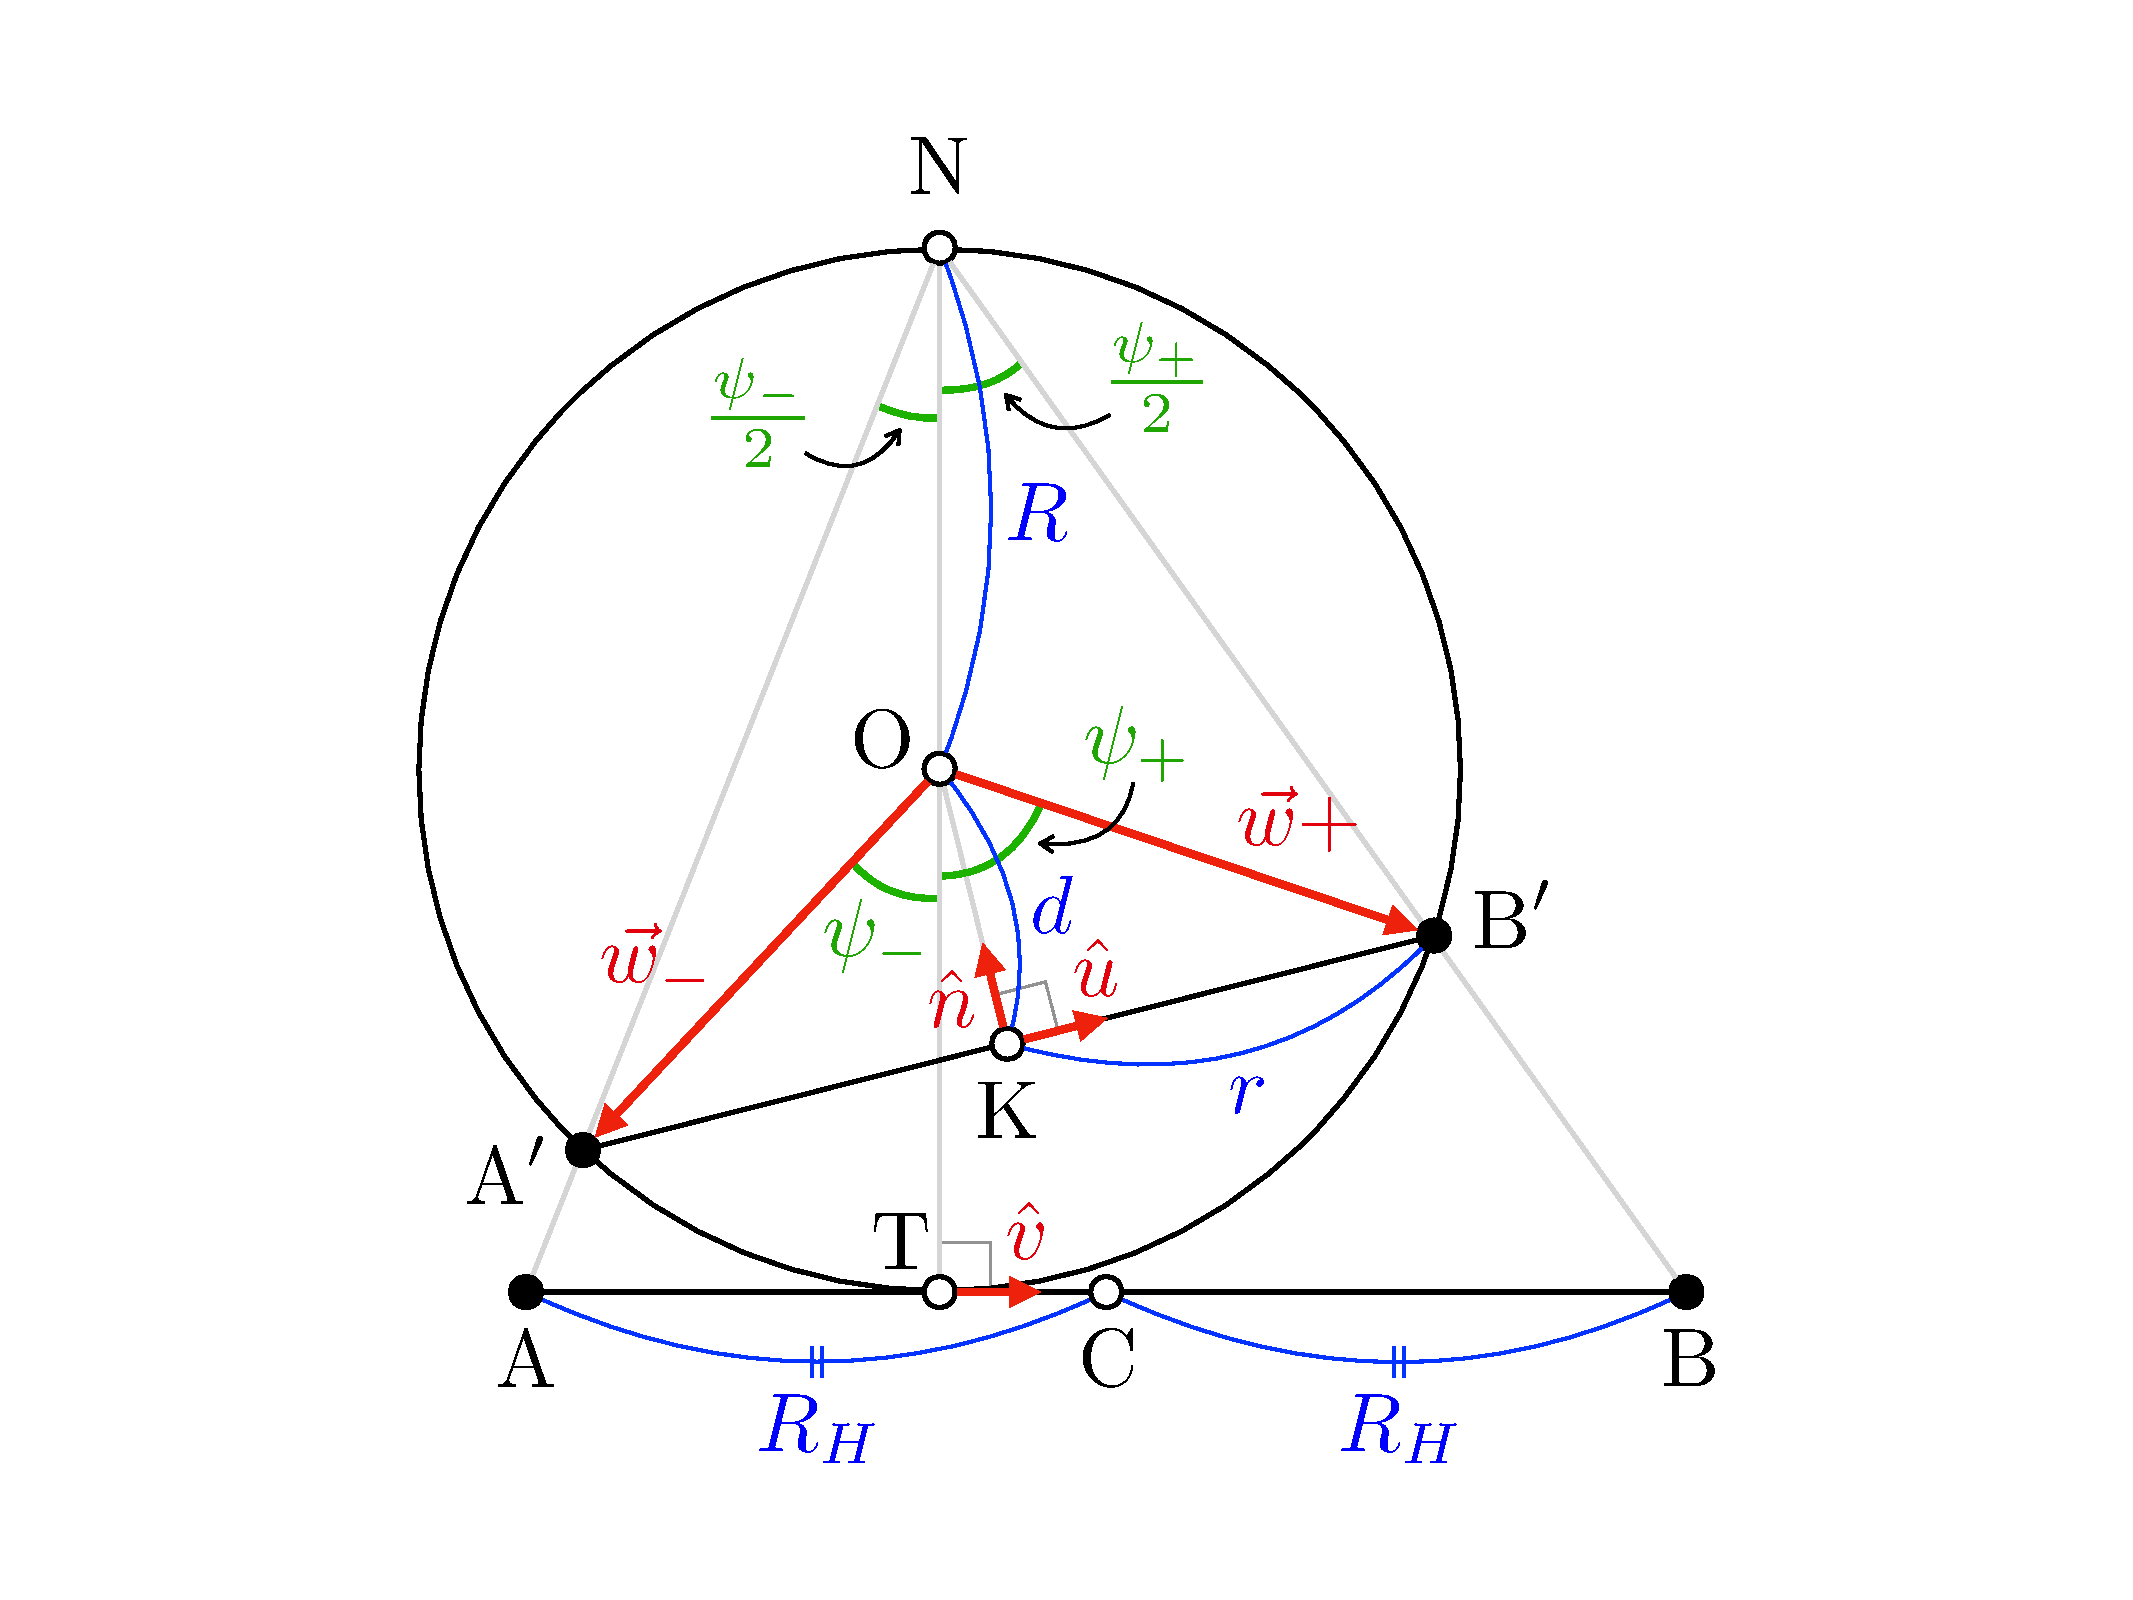
\includegraphics[width=0.8\linewidth]{stereographic_projection.pdf}
\label{sp}
\end{figure}

\begin{eqnarray}
n_xx+n_yy+n_zz = k\\
\end{eqnarray}

\begin{eqnarray}
k &=& \hat{n}\cdot\mathbf{\left<x\right>_M}\\
d &=& \left|k - \hat{n}\cdot \mathbf{x_{RS}}\right|
\end{eqnarray}

\begin{eqnarray}
\hat{u} &=& \frac{l_y\,\vec{l}+m_y\,\vec{m}}{\sqrt{l_y^2+m_y^2}}\\
\hat{v} &=& \frac{u_x^2\,\hat{x} + u_z^2\,\hat{z}}{\sqrt{u_x^2+u_z^2}}\\
\vec{w}_\pm &=& - d\hat{n} \pm \sqrt{R_{RS}^2-d^2}\,\,\hat{u}
%\hat{u} &=& \frac{1}{\sqrt{l_y^2+m_y^2}}\left(l_y\,\vec{l}+m_y\,\vec{m}\right)\\
%\hat{v} &=& \frac{1}{\sqrt{u_x^2+u_z^2}} \left(u_x^2\,\hat{x} + u_z^2\,\hat{z}\right)\\
%\vec{w}_\pm &=& - d\hat{n} \pm \sqrt{R_{RS}^2-d^2}\,\hat{u}
\end{eqnarray}

\begin{eqnarray}
\psi_\pm &=& \arctan{\frac{\left|\hat{v}\cdot w_{\pm}\right|}{w_{\pm,y}}}\\
R_\pm &=& R_{RS} \left( \tan{\frac{\psi_+}{2}} \pm \tan{\frac{\psi_-}{2}} \right)
\end{eqnarray}

\begin{eqnarray}
R_H &=& R_+\\
\mathbf{x_H} &=& R_- \hat{v} + \mathbf{x_{RS}}
\end{eqnarray}



\begin{thebibliography}{}

\bibitem{bestfitplane}
The Math Forum - Line of Best Fit For Points in Three Dimensional Space
(\url{http://mathforum.org/library/drmath/view/69103.html}).

\bibitem{bestfitline}
The Math Forum - Orthogonal Distance Regression Planes (\url{http://mathforum.org/library/drmath/view/63765.html}).

\bibitem{svd}
Singular value decomposition
(\url{https://en.wikipedia.org/wiki/Singular_value_decomposition}).

\end{thebibliography}


\end{document}
